
\documentclass[12pt,a4paper]{article}

\usepackage[T1]{fontenc}
\usepackage[utf8]{inputenc}
\usepackage[polish]{babel}
\usepackage{lmodern}
\usepackage{geometry}
\usepackage{amsmath}
\usepackage{graphicx}

\geometry{margin=2.5cm}

\begin{document}

% ==========================================
% Nagłówek
% ==========================================

\noindent
\begin{minipage}[t]{0.48\textwidth}
    \raggedright
    Jakub Muszka \\
    Nr indeksu: 254822
\end{minipage}
\hfill
\begin{minipage}[t]{0.48\textwidth}
    \raggedleft
    Środa, godz. 12:15 \\
    Data zgłoszenia: 09.11.2026 r.
\end{minipage}

\vspace{0.8cm}

\begin{center}
    {\LARGE\bfseries Komputerowa analiza danych}

    \vspace{0.3cm}

    {\large Zadanie 1}
\end{center}

\vspace{0.5cm}

% ==========================================
% Cel zadania
% ==========================================

\section{Cel zadania}

Zaprezentowanie położenia i zróżnicowania rozkładu
empirycznego oraz współzależności pomiędzy danymi
na przykładzie klasycznego zbioru danych irysów.

% ==========================================
% Wyniki
% ==========================================

\section{Wyniki}

\subsection{Środowisko programistyczne}

Wyniki uzyskano przy użyciu języka Python
w wersji 3.14.8 oraz następujących bibliotek:

\begin{itemize}
    \item pandas -- wersja 3.1.0,
    \item Matplotlib -- wersja 3.11.2.
\end{itemize}

Do obliczeń statystycznych wykorzystano również
własny moduł \texttt{miary\_statystyczne}.
Wykorzystano także moduł \texttt{itertools}
należący do biblioteki standardowej Pythona.

% ==========================================
% Liczebność gatunków
% ==========================================

\subsection{Liczebność gatunków irysów}

\begin{table}[!htbp]
    \centering
    \caption{Liczebność poszczególnych gatunków irysów}
    \label{tab:wyniki}

    \begin{tabular}{|l|c|}
        \hline
        Gatunek & Liczebność (\%) \\
        \hline
        Setosa & 50 (33,33\%) \\
        Versicolor & 50 (33,33\%) \\
        Virginica & 50 (33,33\%) \\
        \hline
        Razem & 150 (100\%) \\
        \hline
    \end{tabular}
\end{table}

% ==========================================
% Miary statystyczne
% ==========================================

\subsection{Miary rozkładu cech irysów}

\begin{table}[!htbp]
    \centering
    \caption{Miary rozkładu dla cech irysów}
    \label{tab:miary}

    \resizebox{\textwidth}{!}{
        \begin{tabular}{|l|c|c|c|c|}
            \hline
            Cecha & Minimum & Śr. arytm. ($\pm$ odch. stand.) & Mediana (Q1--Q3) & Maksimum \\
            \hline
            Długość działki kielicha & 4,3 & 5,84 $\pm$ 0,83 & 5,8 (5,1--6,4) & 7,9 \\
            Szerokość działki kielicha & 2,0 & 3,06 $\pm$ 0,44 & 3,0 (2,8--3,3) & 4,4 \\
            Długość płatka & 1,0 & 3,76 $\pm$ 1,77 & 4,35 (1,6--5,1) & 6,9 \\
            Szerokość płatka & 0,1 & 1,20 $\pm$ 0,76 & 1,3 (0,3--1,8) & 2,5 \\
            \hline
        \end{tabular}
    }
\end{table}

\clearpage

% ==========================================
% Histogramy i boxploty
% ==========================================

\subsection{Charakterystyka rozkładu cech irysów}

Na rysunku \ref{fig:rozklad} przedstawiono
histogramy oraz wykresy pudełkowe
dla czterech analizowanych cech irysów.

\begin{figure}[!htbp]
    \centering
    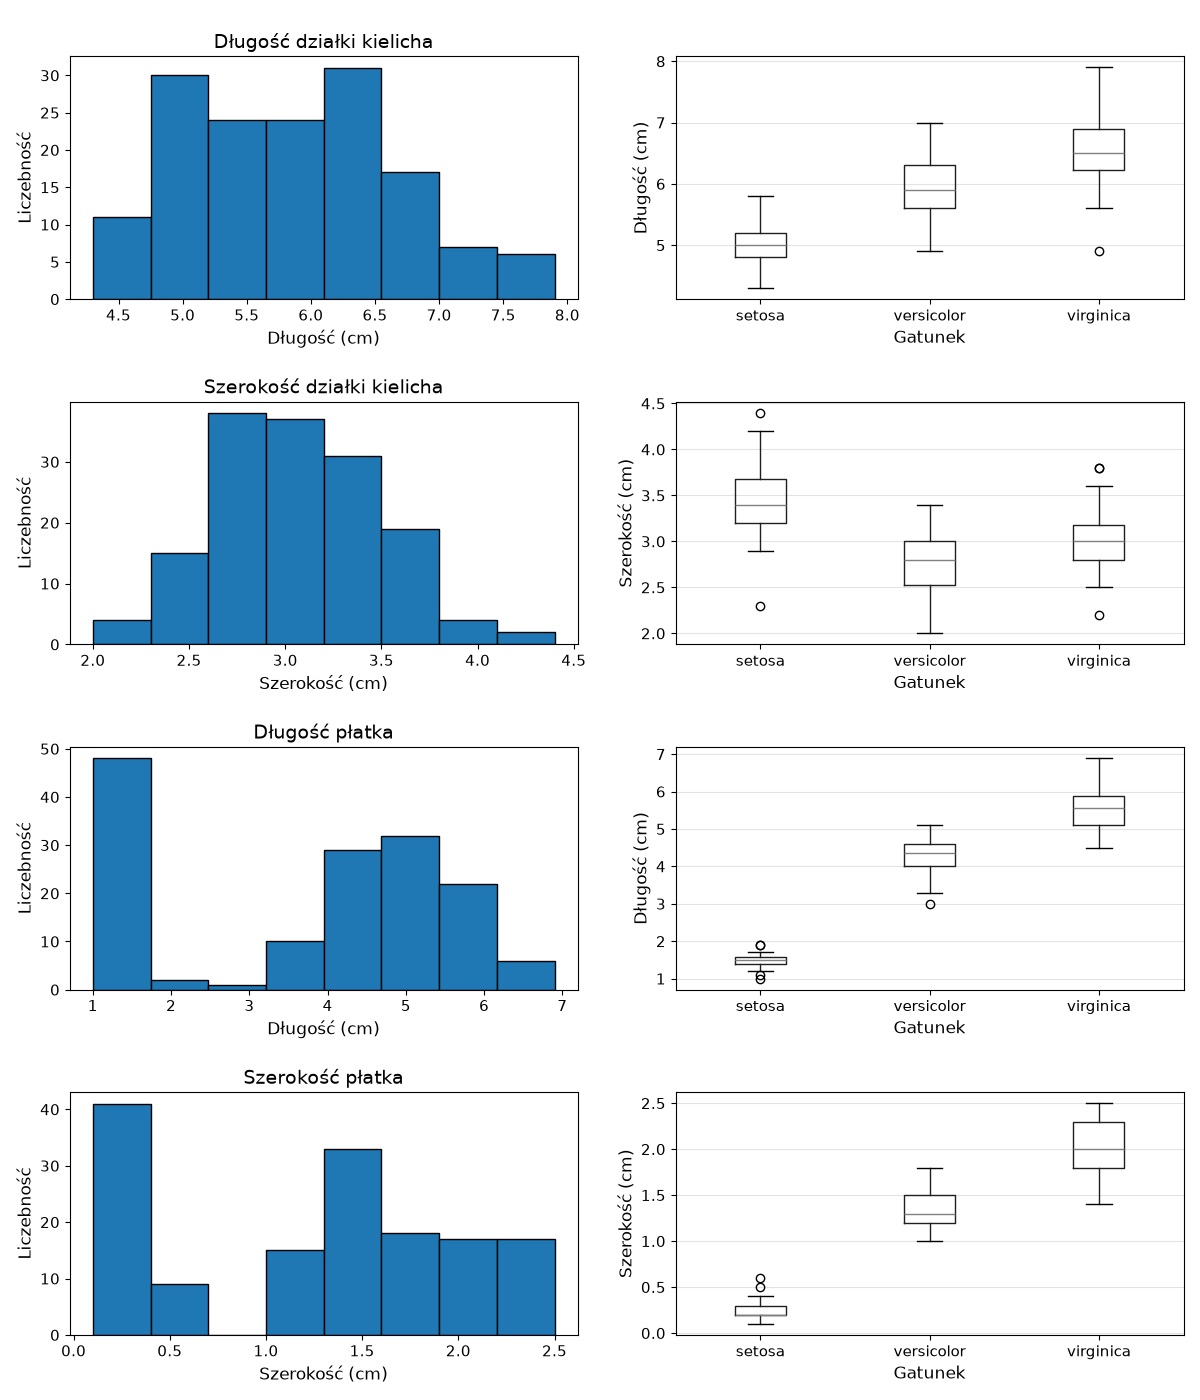
\includegraphics[
        width=\textwidth,
        height=0.70\textheight,
        keepaspectratio
    ]{zdj1.png}

    \caption{Histogramy i wykresy pudełkowe cech irysów}
    \label{fig:rozklad}
\end{figure}

\clearpage

% ==========================================
% Korelacja i regresja
% ==========================================

\subsection{Współzależności pomiędzy cechami irysów}

Na rysunku \ref{fig:korelacja} przedstawiono
wykresy rozrzutu dla wszystkich sześciu par
analizowanych cech wraz z prostymi regresji liniowej.

Dla każdej pary wyznaczono współczynnik
korelacji liniowej Pearsona oraz równanie
prostej regresji liniowej.

\begin{figure}[!htbp]
    \centering
    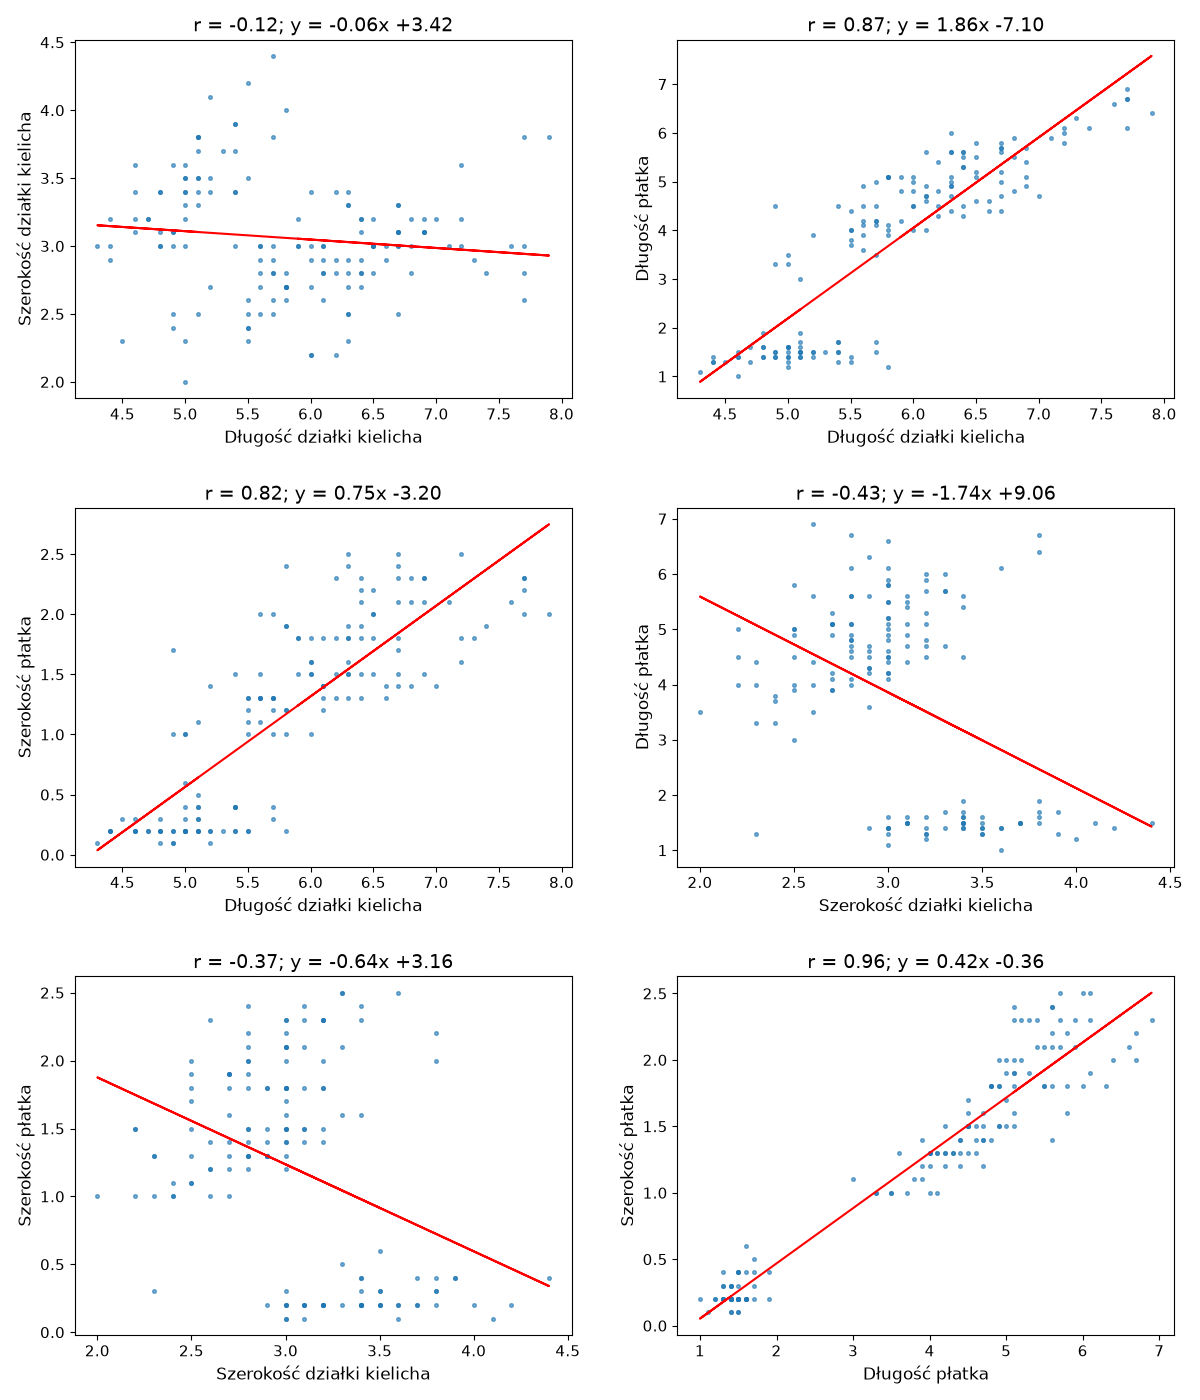
\includegraphics[
        width=\textwidth,
        height=0.70\textheight,
        keepaspectratio
    ]{zdj2.png}

    \caption{Wykresy rozrzutu i regresji liniowej cech irysów}
    \label{fig:korelacja}
\end{figure}

\end{document}
